\FloatBarrier
\section{Operating-point sensitivity and component analysis}
\label{sec:operating_sensitivity-supp20261008}
This analysis reuses the final fitted models and existing calibration and evaluation collections, without further fitting or data generation [\evid{E10}]. The three-hour LightGBM control shares the hybrid's maximum information allowance and is the primary comparator; the zero-hour control supplies context. The hybrid also retains General's immediate alarm path, so the two systems do not have identical decision timing.

A common multiplier $\lambda$ scales the hybrid's original raw branch clean-tail budgets while their relative allocation remains fixed. The 82 settings comprise zero and 81 logarithmically spaced values from $0.01$ to $100$. Order-statistic quantiles of clean calibration scores determine the thresholds; $\lambda=1$ preserves the original thresholds exactly. Alarms require scores strictly above their thresholds, whereas verifier gates retain their at-or-above convention. A zero clean-tail budget can still permit attack-period alarms. Internal routing, verifier cutoffs, the external replay veto and temporal features stay fixed. The verifier's original specialist-score pre-thresholds also stay fixed throughout the $\lambda$ sweep: endpoints outside each fitted candidate region keep the pass-through value of 1, even when the final alarm threshold is lowered. The path therefore describes threshold sensitivity for the retained branch allocation and guards, rather than an exhaustive frontier or an intrinsic hybrid AUPRC.

The calibration clean-FPR caps are $0$, $0.01\%$, $0.025\%$, $0.05\%$, $0.10\%$, $0.25\%$ and $0.50\%$. Each fit selects settings on its pooled calibration collections for two objectives: maximum pooled F1 and maximum worst-family F1. Ties use the other F1 criterion, lower clean FPR, then the stricter setting. Hybrid selection searches the specified path; LightGBM searches its distinct tied-score thresholds exactly. All twenty model/network selections were frozen before this evaluation reanalysis. LightGBM's display curves use clean-calibration quantiles at budgets $0.005\lambda$ on the finite grid; its cap-constrained search is not restricted to that grid.

Figures~\ref{fig:modena_operating_sensitivity-supp20261008} and~\ref{fig:ltown_operating_sensitivity-supp20261008} plot performance against achieved evaluation clean FPR and mark the original operating points. Appendix~\ref{app:operating_sensitivity-supp20261008} gives every cap, objective and achieved calibration/evaluation rate. Means weight the ten-model by six-source cells equally; F1 and nonlinear summaries are calculated within each cell before averaging. Worst-family F1 is consequently the mean of cellwise minima. The protocol was specified after the original evaluation results were known, so these reused sources supply retrospective sensitivity evidence. The original thresholds and research-goal assessment remain unchanged.

Eight diagnostics use the same scores and original thresholds: the full rule, General only, General plus Drift, General plus Noise, specialists only, verifier bypass, external replay-veto removal, and removal of both guards. Remaining branches retain their guards. Removing a specialist's alarms leaves its score channels in the shared router, feedback and verifier inputs; the specialists-only rule does not consume General's output. These are conditional alarm and guard interventions, not separately retrained architectures or measurements of computational savings. Appendix~\ref{app:operating_sensitivity-supp20261008} reports all diagnostic scores. Their interpretation shares the source-reuse and component-identification limits discussed in Chapter~\ref{ch:discussion}.

With pooled-F1 calibration, the hybrid has higher mean pooled F1 at five of seven caps in Modena and six in L-Town. LightGBM leads at the zero cap in both networks and at 0.01\% in Modena; it also has higher random and targeted family means at every cap under both objectives. In Modena, the hybrid improves drift and noise at every positive cap. At the 0.025\% cap, its pooled F1 is 0.8652 versus LightGBM's 0.8503, with evaluation clean FPRs of 0.02705\% and 0.02642\%. The false-positive cost depends on the objective: at the 0.1\% cap under worst-family-F1 calibration, hybrid pooled F1 is 0.8613 versus 0.8240, while its evaluation FPR is lower, 0.07066\% versus 0.10296\%. A common calibration cap therefore permits different evaluation rates, including rates above that cap.

L-Town exposes a replay tradeoff. At the 0.025\% cap under pooled-F1 calibration, hybrid pooled F1 is 0.9127 versus 0.8977, with evaluation clean FPRs of 0.01950\% and 0.01843\%. This reverses the original pooled-F1 ordering, but hybrid replay is now lower: 0.6903 versus LightGBM's 0.7084. Hybrid replay remains lower at all seven caps under this objective. Worst-family-F1 calibration restores its replay advantage at caps of 0.05\% and above. At 0.05\%, hybrid/control replay F1 is 0.7307/0.7091 and pooled F1 is 0.9010/0.8937, while evaluation clean FPR is 0.04675\%/0.03094\%. The original replay advantage thus depends on the selection objective and false-positive allowance.

The branch diagnostics identify complementary contributions at the original thresholds. General alone has pooled F1 of 0.7200 in Modena and 0.8565 in L-Town, compared with 0.8669 and 0.8950 for the full rule. Adding the specialists raises drift/noise F1 from 0.4979/0.4491 to 0.8274/0.8439 in Modena and from 0.8149/0.7877 to 0.8990/0.9279 in L-Town. Specialists alone retain strong drift/noise scores but reach replay F1 of only 0.0234 and 0.1103. The full rule has higher pooled F1 than every branch-removal variant in all 60 cells of each network. It nevertheless sacrifices L-Town replay performance: General alone reaches 0.7411 and General plus Drift reaches 0.7416, compared with 0.7312 for the full rule. Omitting Noise alarms improves replay in 58 cells and leaves it unchanged in two, while reducing pooled and noise F1 in all 60.

Bypassing the verifier reduces pooled F1 to 0.6737 in Modena and 0.7273 in L-Town. Clean FPR rises from 0.0584\% to 0.4578\% and from 0.0550\% to 0.3409\%, respectively; pooled F1 falls and clean FPR rises in all 60 cells of both networks. Modena's family macro F1 changes much less, from 0.9045 to 0.9019, because its family-conditioned populations omit much of the clean-period background counted by pooled F1. These results establish the verifier's alarm-filtering contribution with its fitted inputs fixed, without isolating the value of its early-warning features.

The external replay veto has a smaller effect while verification remains active. Removing it changes Modena pooled/replay F1 to 0.8663/0.9219 and L-Town to 0.8946/0.7281. L-Town noise F1 instead increases from 0.9279 to 0.9304. Removing both guards lowers pooled/replay F1 further, to 0.6643/0.7927 and 0.7136/0.6518. The larger replay losses after verification is bypassed show that guard effects depend on one another; they cannot be added as independent contributions. General's internal routing is unchanged wherever General alarms contribute. The repeated directions across cells describe the six shared source collections, rather than 60 independent data replications.

\begin{figure}[p]
\centering
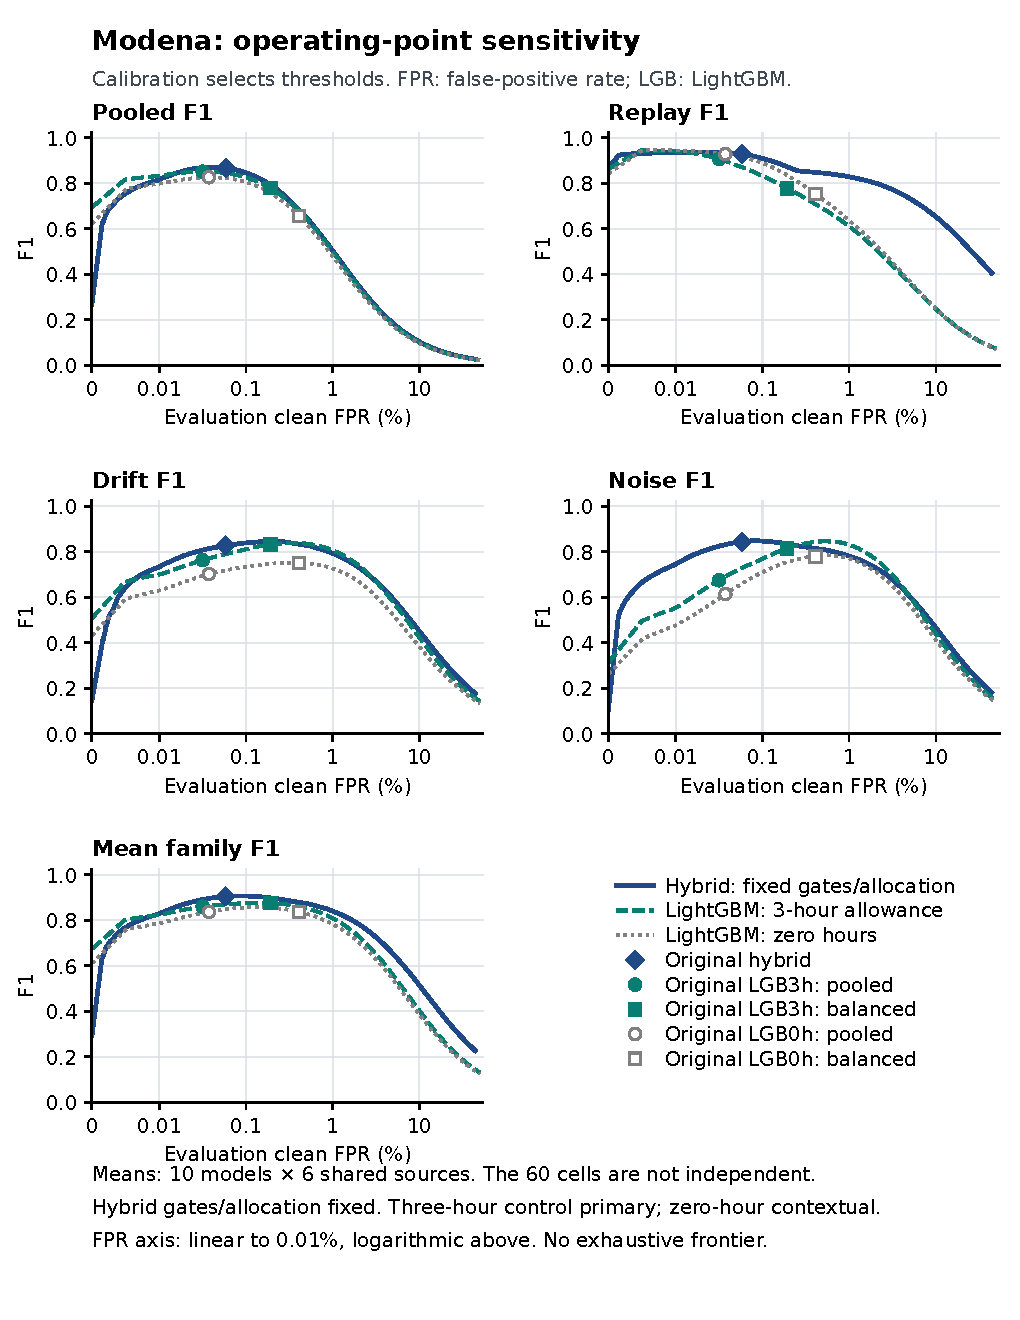
\includegraphics[width=\linewidth,height=.82\textheight,keepaspectratio]{figures/modena_operating_point_sensitivity.pdf}
\caption[Modena operating-point sensitivity]{Modena operating-point sensitivity on the existing evaluation sources. Curves follow the specified calibration-derived threshold paths; symbols mark original operating points. The horizontal axis shows achieved evaluation clean false-positive rate (FPR) in percent, with a linear region up to $0.01\%$ and logarithmic scaling above it. All points are equal-weight means over 60 shared model/source cells. The hybrid path fixes branch allocation and all guard settings.}
\label{fig:modena_operating_sensitivity-supp20261008}
\end{figure}
\begin{figure}[p]
\centering
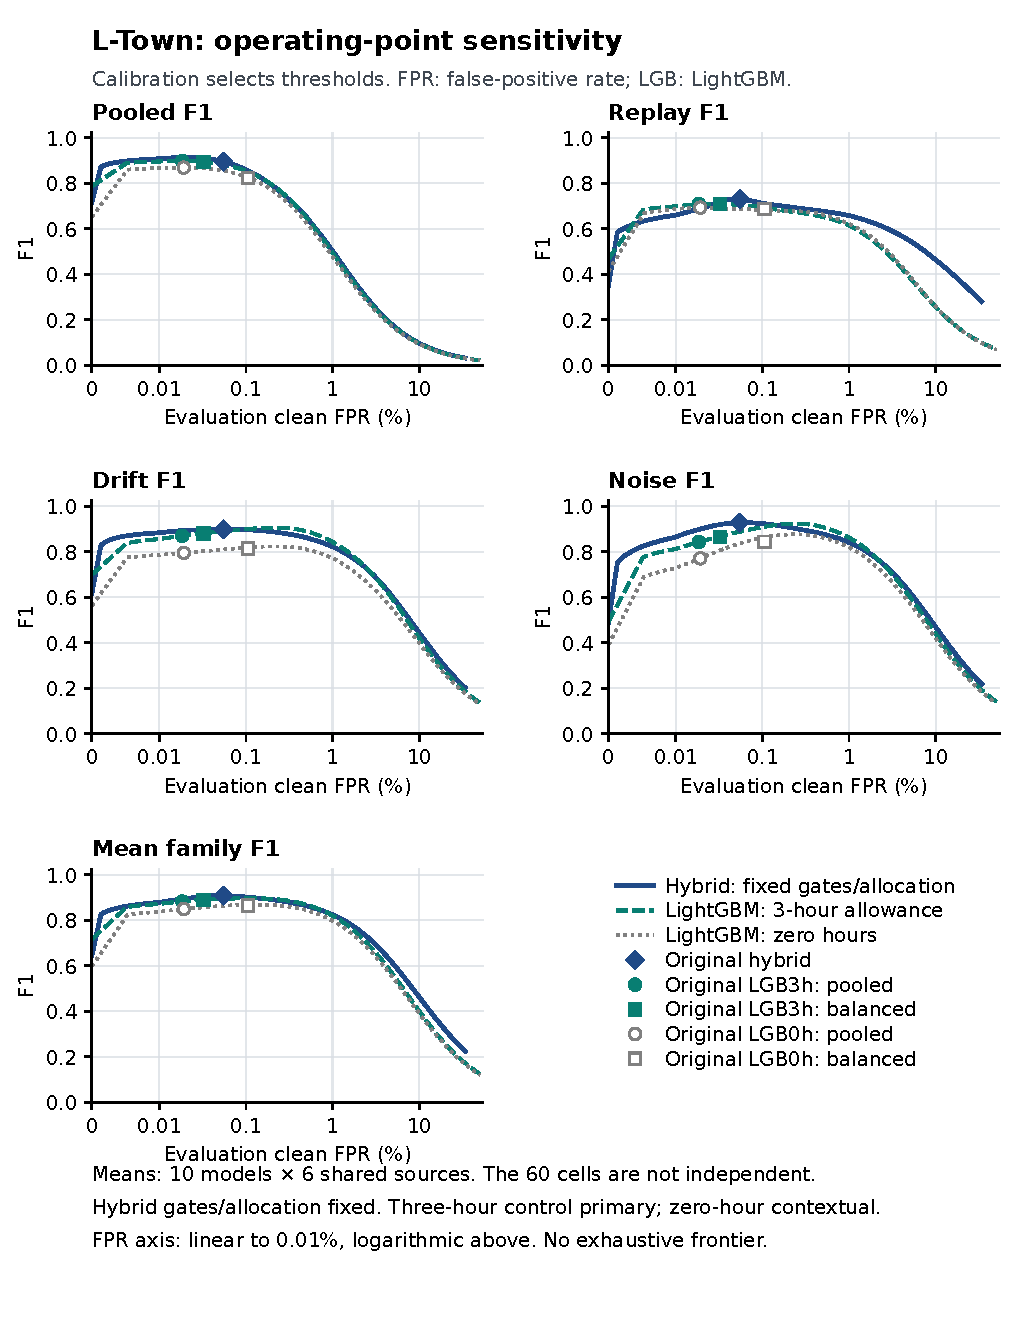
\includegraphics[width=\linewidth,height=.82\textheight,keepaspectratio]{figures/ltown_operating_point_sensitivity.pdf}
\caption[L-Town operating-point sensitivity]{L-Town operating-point sensitivity under the same supplementary protocol. Evaluation clean FPR is observed separately from the calibration cap. The three-hour LightGBM control is primary; the zero-hour control supplies timing context. Curves are finite threshold paths, not an exhaustive hybrid frontier. All points average 60 shared model/source cells.}
\label{fig:ltown_operating_sensitivity-supp20261008}
\end{figure}
\FloatBarrier
